\documentclass[tikz,border=0pt]{standalone}
  \usepackage{amsmath,amsfonts}
  \usepackage{xspace}
  \usepackage{xcolor}
  \usepackage{amsmath,amsfonts,xcolor,xspace}
%% notation
  \newcommand{\vct}{\mathbf}     % vectors
  \newcommand{\uvc}[1]{\hat{\mathbf{#1}}} % unit vectors
  \newcommand{\dtkn}[2]{\Delta_{#1,#2}} % angle difference
  %% variables
  % unit vectors
  \newcommand{\er}{\uvc{e}_r}      % e_r
  \newcommand{\et}{\uvc{e}_\theta} % e_theta
  \newcommand{\erk}[1]{\uvc{e}_{r_{#1}}}      % e_r
  \newcommand{\etk}[1]{\uvc{e}_{\theta_{#1}}} % e_theta
  \newcommand{\Der}{\dot{\uvc{e}}_r}      % e_r dot
  \newcommand{\Det}{\dot{\uvc{e}}_\theta} % e_theta dot
  \newcommand{\ei}{\uvc{e}_i}      % e_i
  \newcommand{\ej}{\uvc{e}_j}      % e_j
  \newcommand{\eik}[1]{\uvc{e}_{i_{#1}}}      % e_i
  \newcommand{\ejk}[1]{\uvc{e}_{j_{#1}}}      % e_j
  % other vectors
  \newcommand{\nf}{F}              % Generic force name
  \newcommand{\vf}{\vct{\nf}}      % Generic force vector
  \newcommand{\nt}{T}              % Tension name
  \newcommand{\ntk}[1]{T_{#1}}              % Tension name
  \newcommand{\vt}{\vct{\nt}}      % Tension vector
  \newcommand{\vtk}[1]{\vct{\nt}_{#1}}      % Tension vector
  \newcommand{\vg}{\vct{g}}        % Gravity vector
  \newcommand{\ro}{\vct{r}_{o}}    % Pivot position
  \newcommand{\vo}{\vct{v}_{o}}    % Pivot velocity
  \newcommand{\ao}{\vct{a}_{o}}    % Pivot acceleration
  \newcommand{\rok}[1]{\vct{r}_{o_{#1}}}    % Pivot position
  \newcommand{\vok}[1]{\vct{v}_{o_{#1}}}    % Pivot velocity
  \newcommand{\aok}[1]{\vct{a}_{o_{#1}}}    % Pivot acceleration
  \newcommand{\aox}{a_{ox}}        % Pivot x acceleration
  \newcommand{\aoy}{a_{oy}}        % Pivot y acceleration
  \newcommand{\vr}{\vct{r}}        % Mass position
  \newcommand{\vv}{\vct{v}}        % Mass velocity
  \newcommand{\va}{\vct{a}}        % Mass acceleration
  \newcommand{\allt}{\mathbb{T}}
  \newcommand{\allq}{\vct{v}_{\theta}}
  \newcommand{\allqd}{\vct{v}_{\dot\theta^2}}
  \newcommand{\allqdd}{\vct{v}_{\ddot\theta}}
  \newcommand{\ws}{\vct{w}_s}
  \newcommand{\wc}{\vct{w}_c}
  \newcommand{\allti}{(\mathbb{T})_{i}}
  \newcommand{\allqi}{(\vct{v}_{\theta})_{i}}
  \newcommand{\allqdi}{(\vct{v}_{{\dot\theta^2}})_{i}}
  \newcommand{\allqddi}{(\vct{v}_{{\ddot\theta}})_{i}}
  \newcommand{\wsi}{{(\vct{w}_s})_{i}}
  \newcommand{\wci}{{(\vct{w}_c})_{i}}
  \newcommand{\A}{A}
  \newcommand{\B}{B}
  \newcommand{\C}{C}
  \newcommand{\D}{S}
  %% text
  \newcommand{\ntsp}{not-too-simple\xspace}
  %% others
  \newcommand{\todo}[1]{\textcolor{red}{#1}}

\usetikzlibrary{quotes,angles}
\begin{document}
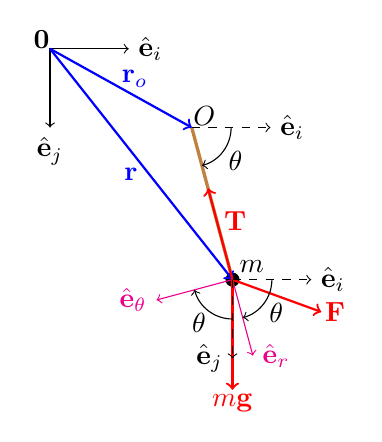
\begin{tikzpicture}[yscale=-1]
  \draw [<->]
    (1,0) coordinate (i) node[right] {$\ei$}
    -- (0,0) coordinate (o) node[above left,inner sep=0pt] {$\vct{0}$}
    -- (0,1) coordinate (j) node[below] {$\ej$};

  \draw[very thick,brown]
    (1.8,1.0) coordinate (ro) node[black,above right,inner sep=0pt] {$O$}
    -- ++(75:2) coordinate (rm) node[black,above right,inner sep=2pt] {$m$} node[black,circle,inner sep=1.8pt,fill]{};
  \draw [->,blue,thick]
    (o) -- node[above right, inner sep=0pt]{$\ro$} (ro);
  \draw [->,blue,thick]
    (o) -- node[below left, inner sep=1pt]{$\vr$} (rm);
  \draw [<->,magenta]
    (rm)++(75:1) coordinate (er) node[right] {$\er$}
    -- (rm) -- ++(165:1) coordinate (et) node[left] {$\et$};
  \draw [dashed,->]
    (ro) -- ++(1,0) coordinate (roei) node[right] {$\ei$};
  \pic["$\theta$", draw=black, <-, angle eccentricity=1.4, angle radius=0.5cm]
    {angle=er--ro--roei};

  %% Forces
  \draw [->,red,thick]
    (rm) --  node[above right,inner sep=1pt] {$\vt$} ++(75:-1.2) coordinate (t);
  \draw [->,red,thick]
    (rm) -- ++(20:1.2) coordinate (f) node[right,inner sep=1pt] {$\vf$};
  \draw [->,red,thick]
    (rm) -- ++( 0,1.4) coordinate (f) node[below,inner sep=1pt] {$m\vg$};
  %% Copy of {ei,ej} at m
  \draw [dashed,->]
    (rm) -- ++(1,0) coordinate (rmei) node[right] {$\ei$};
  \draw [dashed,->]
    (rm) -- ++(0,1) coordinate (rmej) node[left] {$\ej$};
  \pic["$\theta$", draw=black, <-, angle eccentricity=1.4, angle radius=0.5cm]
    {angle=er--rm--rmei};
  \pic["$\theta$", draw=black, <-, angle eccentricity=1.4, angle radius=0.5cm]
    {angle=et--rm--rmej};
  
\end{tikzpicture}
\end{document}